\documentclass[10pt,a4paper,oneside]{report}
\usepackage[utf8]{inputenc}
%Algemene documentinstellingen als dubbelzijdig, codering, rapportsoort etc.

\usepackage[dutch]{babel}
\usepackage[backend=biber,style=apa,sorting=nty,natbib]{biblatex}
\addbibresource{bibliografie.bib}
\DeclareLanguageMapping{dutch}{dutch-apa}
%APA-richtlijnen en taalinstellingen

\usepackage{afterpage}
\newcommand\blankpage{
    \null
    \thispagestyle{empty}
    %\addtocounter{page}{-1} %Weggehaald zodat paginanummer blijft doortellen op lege pagina's
    \newpage}
%Code om blanke pagina's in te voegen
%Code is \afterpage{\blankpage}

\usepackage{graphicx}
\graphicspath{ {./Images/} }
%Om figuren in te voegen

\usepackage{fancyhdr} %Voet- en kopteksten
\usepackage{csquotes} %Quotes die Babel respecteren
\usepackage{lastpage} %Variabele voor paginanummering (om te zeggen bijv. pagina 5 van 63)
\usepackage{booktabs} %Tabeloptimalisatie en opmaak
\usepackage{pdfpages} %Samenvoegen van PDF's 
\usepackage{lipsum} %Lorem ipsum
\usepackage{color} %Tekstkleur
\usepackage{microtype} %Tegen de underfull errors en om justifying te helpen
\usepackage[pages=some]{background} %Achtergrondafbeeldingen bij voorwoord
\usepackage{comment} %Om delen van de tekst uit te schakelen
\usepackage{titling} %Titels voor op de titelpagina
\usepackage{changepage} %Horizontale marges tijdelijk veranderen op de titelpagina

\usepackage[linktoc=all]{hyperref}
\hypersetup{
    colorlinks=true,
    linkcolor=black,
    filecolor=cyan,
    urlcolor=cyan,
    citecolor=black,
    breaklinks=true,
    bookmarksopen=true}
%Links naar websites, bronnen, inhoudsopgave, pagina's etc.

\def\titel{Procesverslag Gerrit Post}
\def\ondertitel{Proces- en reflectieverslag voor de afstudeeropdracht bij Seafood Connection B.V. te Urk}
\def\auteur{Gerrit Post}
\def\studentklas{S1071236 --- AC4V}
\def\mailstudent{S1071236@student.windesheim.nl}
\def\telstudent{+31 642 678 172}
\def\school{Hogeschool Windesheim}
\def\domein{Accountancy, BMR}
\def\mailschool{a.vanden.brandhof@windesheim.nl}
\def\organisatie{Seafood Connection B.V.}
\def\mailorganisatie{info@seafoodconnection.nl}
\def\telorganisatie{+31 527 687 066}
\def\docent{Drs. A. Dannenberg RA}
\def\begeleidereen{J.J. Molenaar, MSc.}
\def\begeleidertwee{L. Brouwer}
\def\datum{7 januari 2019} %Alle variabelen in het document als titel, datum etc.
\newcounter{bijlage}[section] %Om het aantal bijlages bij te houden

\title{\titel}
\author{\auteur}
\date{\datum}
%Documenteigenschappen worden hier gekopieerd uit Definities.tex

%---------------------------EIND VAN PREAMBLE---------------------------




\begin{document}
%%Dit document is om direct te importeren in main.tex

\begin{titlepage}
    \begin{adjustwidth*}{-2cm}{-2cm}
    \vspace*{-3.5cm}
    \hspace{12cm}
    \includegraphics[width=0.4\textwidth]{download} \\
    \begin{center}
    \vspace*{3cm}
    {\Huge\thetitle}
    
    \vspace*{0.4cm}
    \textnormal{\ondertitel}
    
    \vspace{5cm}
    \textbf{Door} \\
    \theauthor \\
    \studentklas \\
    \mailstudent \\
    \telstudent \\
    
    \vspace{0.7cm}
    \textbf{Onderwijsinstituut} \\
    \school \\
    \domein \\
    \mailschool \\
    
    \vspace{0.7cm}
    \textbf{Organisatie} \\
    \organisatie \\
    \mailorganisatie \\
    \telorganisatie \\

    \vspace{0.7cm}
    Afstudeerdocent: \docent \\
    1\textsuperscript{e} Afstudeerbegeleider: \begeleidereen \\
    2\textsuperscript{e} Afstudeerbegeleider: \begeleidertwee \\

    \vspace{0.7cm}
    \textbf{Datum} \\
    \thedate
    \end{center}
    \end{adjustwidth*}
\end{titlepage}
%Titelpagina
 %Dit kan alleen als de preamble hetzelfde is
\includepdf{./Titelpagina/titelpagina.pdf}
%Titelblad wordt geïmporteerd als PDF want die is oneside en dit document twoside, zie eerste regel

\afterpage{\blankpage}
\backgroundsetup{contents=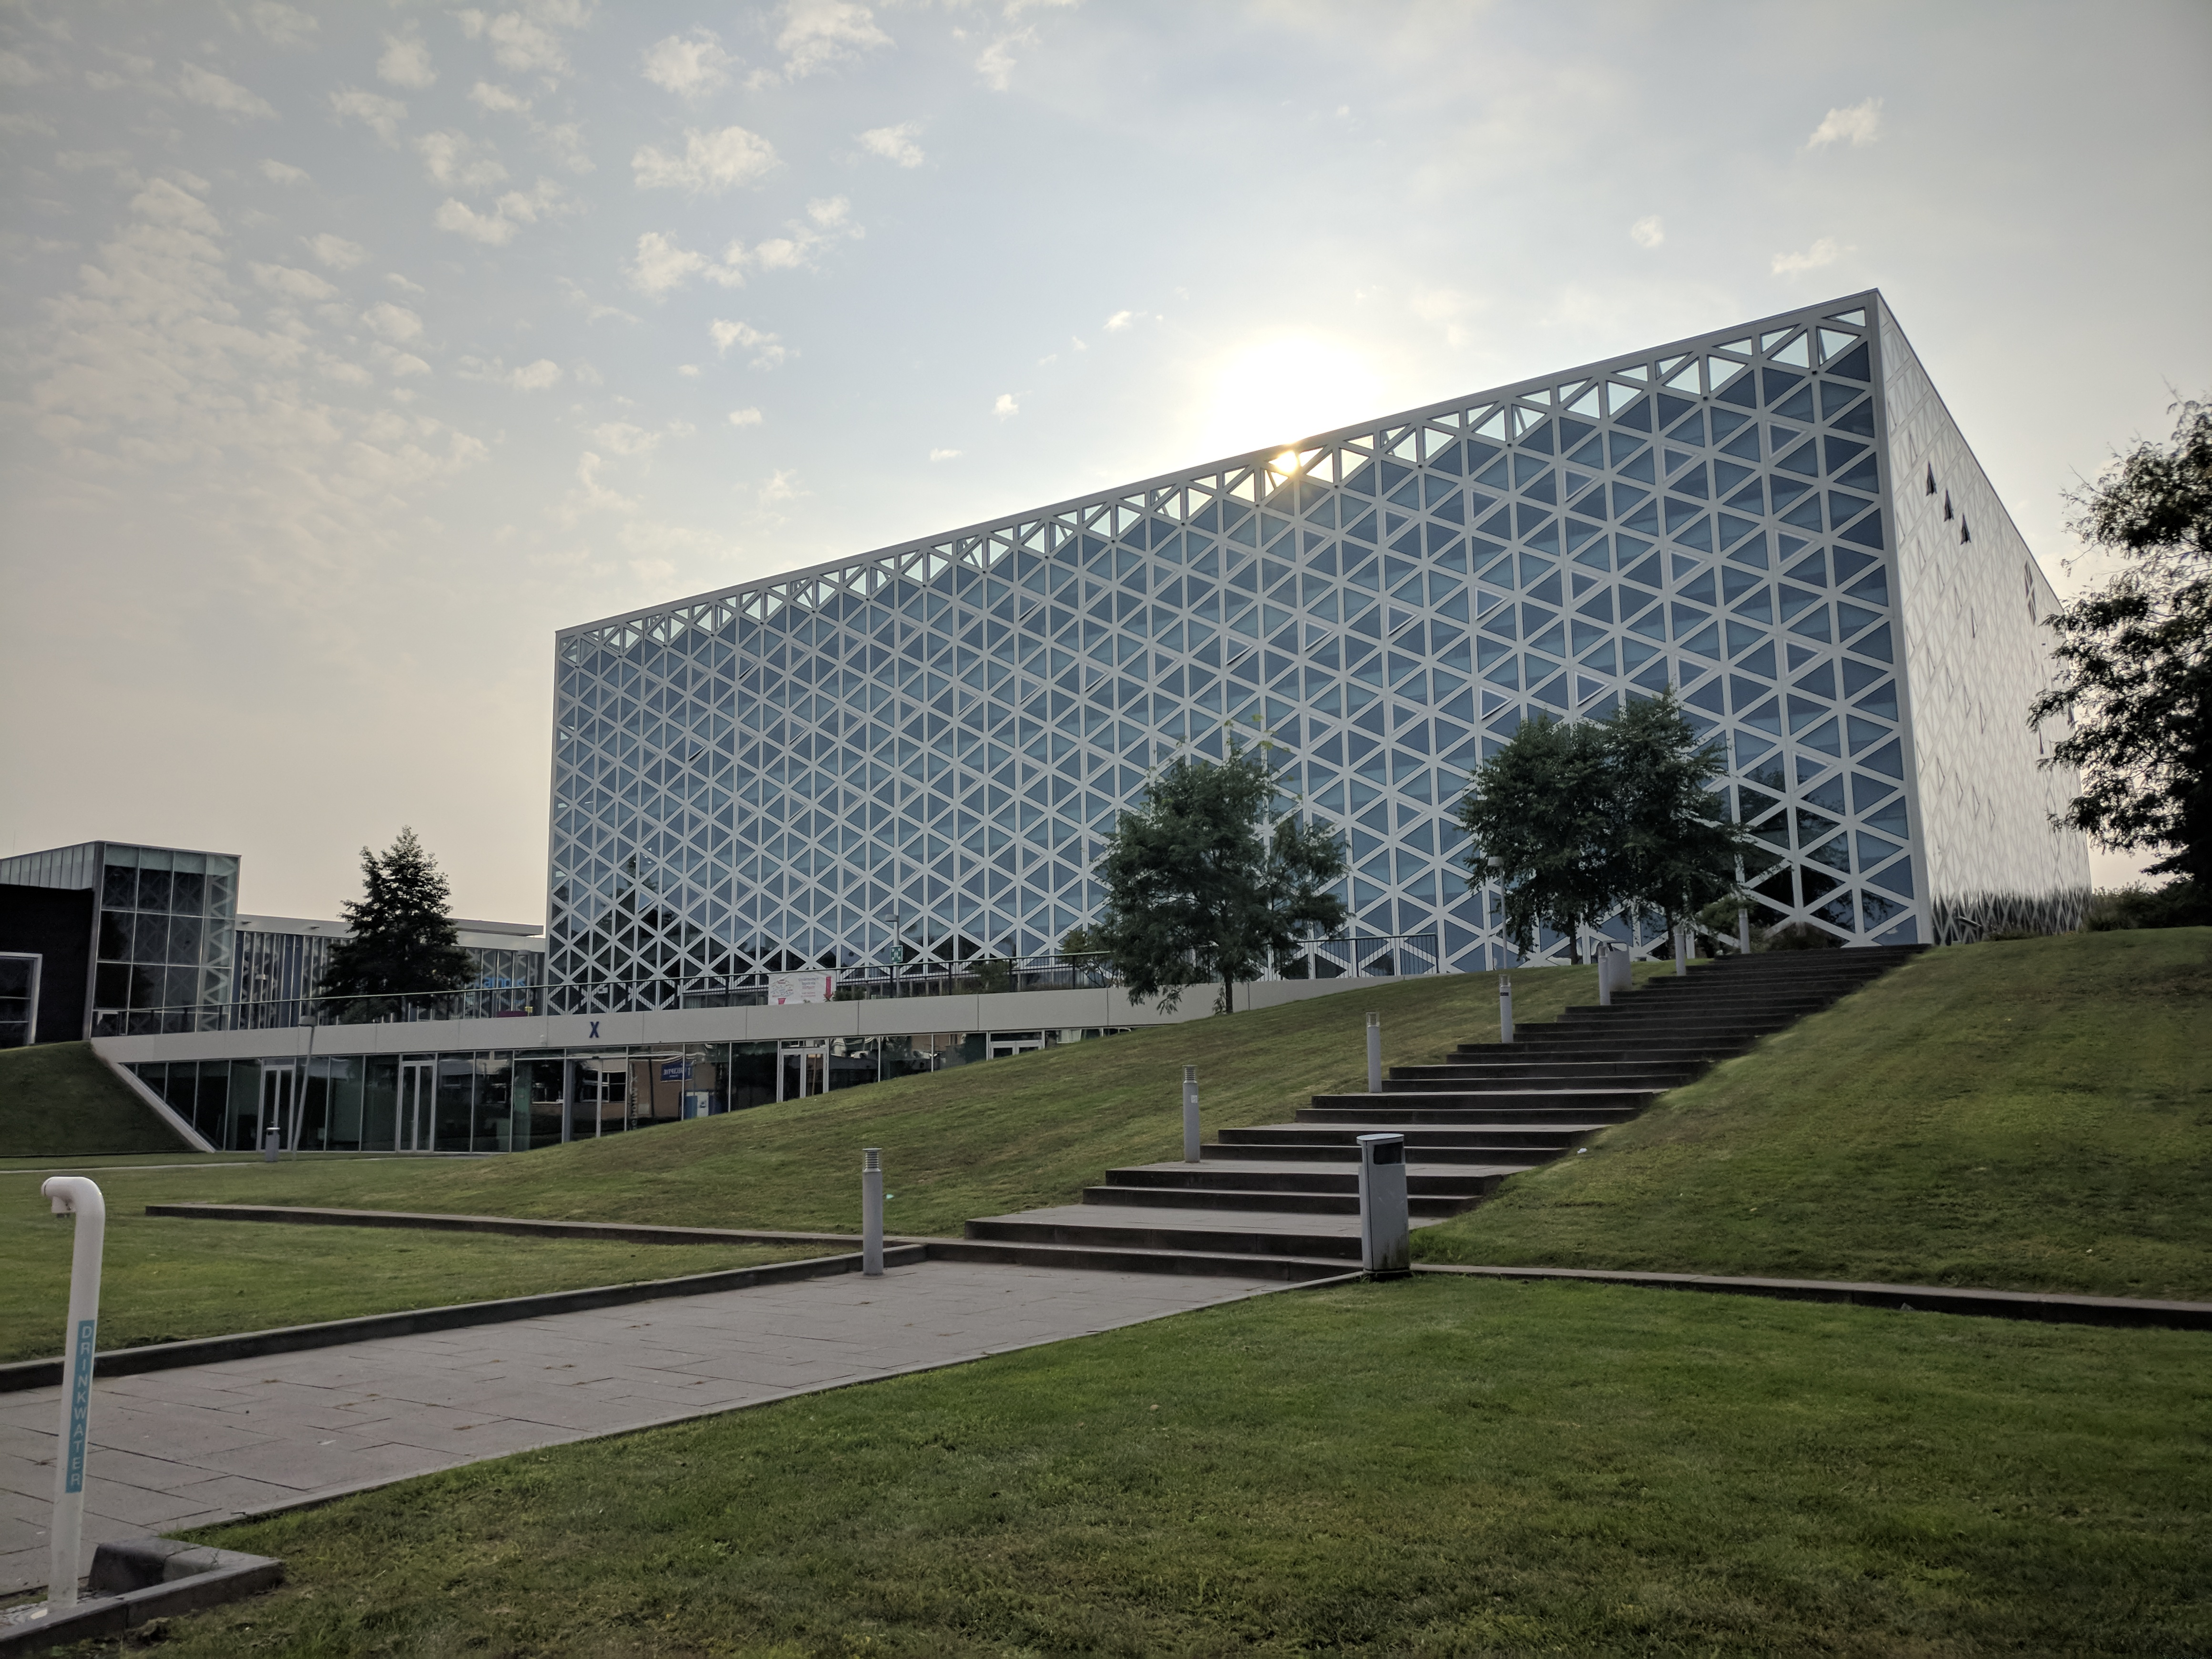
\includegraphics{windesheim},angle=0,scale=0.3,opacity=1,hshift=700}
\BgThispage
%Na titelblad een lege pagina zodat er niets op de achterkant staat als hij dubbelzijdig wordt geprint

\chapter*{Voorwoord}
\thispagestyle{empty}
\backgroundsetup{contents=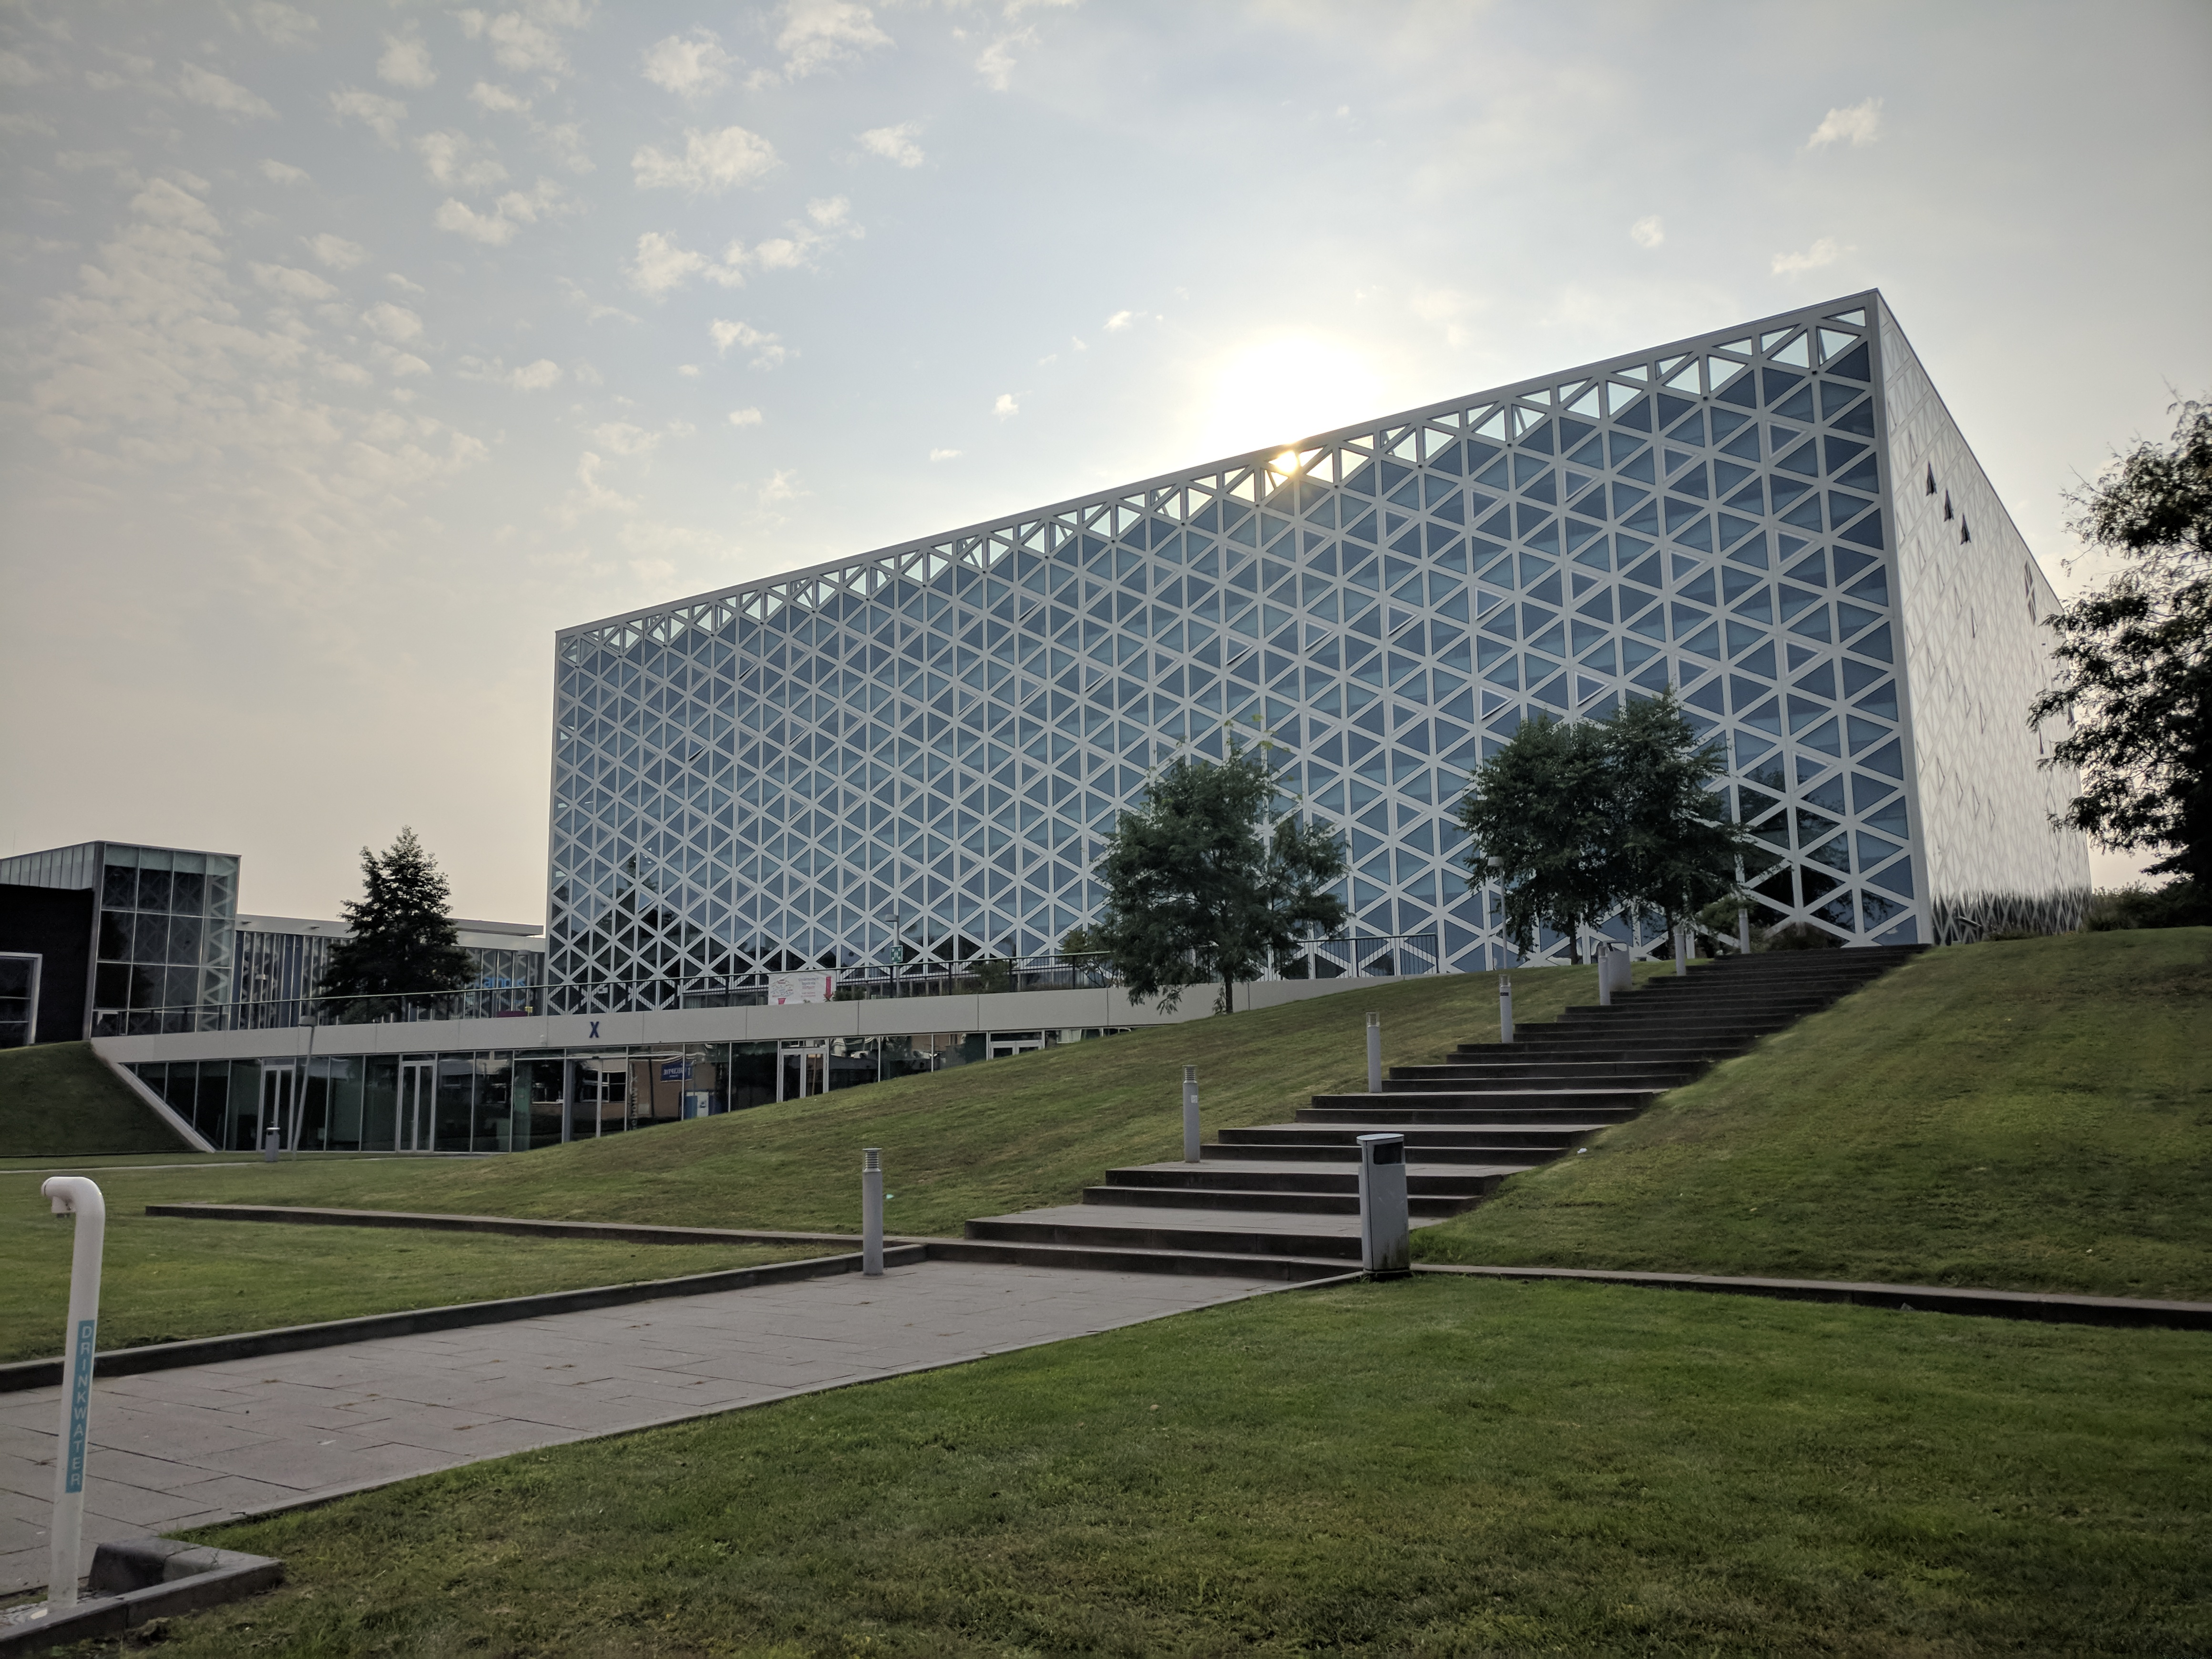
\includegraphics{windesheim},angle=0,scale=0.3,opacity=0.5,hshift=-1300}
\BgThispage
Het maken van een afstudeerproduct is een logische en verplichte laatste stap voor het afronden van mijn bacheloropleiding aan de Windesheim te Zwolle. Al voor de opdracht van start was gegaan was ik zeer geïnteresseerd om deze afstudeerstage uit te kunnen voeren bij een uitdagende en atypische opdrachtgever. Dit verlangen was vooral gegrond in het feit dat ik een affiniteit voor AO/BIV aan het ontwikkelen was en graag wilde toetsen of mijn kennis op dit vakgebied voldoende is. En waar beter deze kennis te toetsen dan bij een werkgever waar niet zomaar de geleerde typologieën gekopieerd en geplakt kunnen worden?
Mijn zoektocht begon naar een organisatie die in dit profiel past en graag met mij samen zou willen werken aan een nuttig eindproduct.

Eind juni kwam ik op de tennisbaan in gesprek met oud-collega Jurian, hier kwam Seafood Connection ter sprake als een interessante organisatie voor mij als afstudeerder. Al snel zat ik aan tafel met CFO Lucas Brouwer en voorgenoemde Jurian Molenaar waar Seafood Connection een steeds interessantere kandidaat leek te worden. Ik ben blij met de samenwerking die wij zijn aangegaan en ik hoop op een vruchtbare en productieve afstudeerperiode. Een bijzondere dank aan Rienk Bouma, Jon Bergsma, en Alidus Dannenberg voor de begeleiding vanuit school bij het formulerende proces van de opdracht. 

Ik wens de lezer veel plezier bij het lezen van dit afstudeerwerkplan en vanzelfsprekend ben ik bereid om vragen te beantwoorden en mee te nemen voor de opdracht.

\bigskip
\noindent
\textbf{Gerrit Post} \\
\textit{Student Accountancy, Hogeschool Windesheim}
%Voorwoord met achtergrondafbeelding


\chapter*{Samenvatting}
\thispagestyle{empty}
\lipsum[1-4]

\setcounter{page}{4} %Door importeren van PDF klopt paginanummer niet, hierbij gecorrigeerd
\tableofcontents
\thispagestyle{empty}

\chapter*{Inleiding}
\addcontentsline{toc}{chapter}{Inleiding} %Ongenummerde chapters komen niet in de ToC, met deze code wel
Om duidelijk de uit te voeren opdracht te definiëren en te verkennen wordt in dit verslag met een brede blik gekeken de probleemformulering, -omgeving, en er wordt onderzocht wat er concreet gaat spelen bij dit onderzoek. In samenwerking met de finance afdeling van Seafood Connection (hierna als afkorting: SFC) wordt georiënteerd op de opdrachtformulering en wordt ook de opdrachtomgeving bekeken aan de hand van een uitgebreide bedrijfsverkenning. 

Om de lezer een goed beeld te geven van de opdrachtomgeving wordt eerst uitgebreid, maar doelgericht, de bedrijfsachtergrond beschreven. Vervolgens wordt de eerste stap van de onderzoekscyclus uitgewerkt volgens het model van Nel Verhoeven waar de probleemomschrijving breed en diep wordt uitgewerkt. In hoofdstuk drie wordt dit probleem omgezet in een concreet ontwerp waarin concreet wordt nagedacht over de invulling van de afstudeeropdracht- en periode. De competentieontwikkeling in hoofdstuk vier beschrijft de manier waarop de afstudeerstagiair gaat werken aan de competentie- en ontwikkelingspunten. Als slot vindt u de bronnenlijst, de bijlagen die verdiepend zijn voor dit plan, en de tijdsplanning voor de afstudeerperiode. 



\chapter{Competentieontwikkeling}
    \section{Persoonlijke ontwikkelpunten}
Ten behoeve van het persoonlijk functioneren en ontwikkelen voor de afronding van de bachelor opleiding accountancy, zijn de volgende ontwikkelpunten geformuleerd:
\begin{enumerate}
    \item Er worden stappen gezet om de communicatieve vaardigheden in woord en geschrift te versterken door voor interviews (met zowel de opdrachtgever als andere betrokkenen) goed na te denken over welke informatie benodigd is en hoe deze op een zo'n neutraal mogelijke wijze kan worden geformuleerd. Taalgebruik in rapportage wordt verbeterd door meerdere reviewers te vragen kritisch te kijken naar de rapportage en te doorgronden welke fouten worden gemaakt om verdere fouten te voorkomen. 
    \item Er wordt volgens een vast tijdsplan gestudeerd en gewerkt zodat er een dwangmatige urgentie is om door te blijven werken. Dit wordt gerealiseerd door vaste routines op te bouwen en periodieke mijlpalen te stellen. Periodieke reflectie op de mijlpalen is hier ook belangrijk.
    \item Er wordt beter nagedacht over de toegevoegde waarde richting een potentiële werkgever en deze wordt op een eenduidige wijze geformuleerd. Dit wordt bereikt door te werken aan zo veel mogelijk werkzaamheden die relevant zijn met de accountancy opleiding als achtergrond. Concreet moet worden geformuleerd welke waarde kan worden toegevoegd die een andere afgestudeerde AC-student niet zou kunnen aanbieden.
\end{enumerate}

\newpage
    \section{Landelijke beroepscompetenties}
Op de Windesheim community zijn een aantal onderzoekscompetenties geformuleerd om de afstudeerstudent te helpen bij het succesvol afronden van de scriptie. Een aantal hier van hebben betrekking op dit afstudeerwerkplan. Hier wordt verder toegelicht hoe deze competenties aan de orde zijn gekomen bij het opstellen van het AWP. \\
De afgestudeerde bachelor AC-student is in staat om: 
\begin{enumerate}
    \item Een probleemstelling te formuleren
    \item Voor de oplossing van het probleem beschikbare kennis te identificeren
    \item De kwaliteit van de kennis en de theorie die hem ter beschikking staat kritisch te beoordelen
    \item De basis van zijn analyse te modelleren
\end{enumerate}

\noindent
\textit{Ad. 1.} Er is hard en lang over de probleemstelling en aanleiding gediscussieerd met de opdrachtgever en gedeeltelijk met begeleidende docenten. De aanleiding was in de eerste fase van de opdrachtsformulering niet helemaal helder en er moest geschaafd en bijgesteld worden om een goede aanleiding en probleemomschrijving te formuleren. Het lijkt aan de ene hand tegenstrijdig, omdat wel meteen duidelijk was wat de doelstelling was en welke producten opgeleverd moeten worden. Juist door zo hard te denken over de probleemstelling in samenwerking met de betrokken partijen, is de huidige probleemstelling zo hard en onderbouwd. 

\bigskip
\noindent
\textit{Ad 2.} Alvorens het afstudeerwerkplan is opgesteld is er diep en breed gezocht naar enigszins relevante informatie uit een groot aantal soorten bronnen. Andere scripties, toegewijde vakliteratuur, en handreikingen vanuit het opleidingsinstituut waren hier het meest behulpzaam. De term \textit{treasury} (zie paragraaf \ref{def:treasury}) was voor deze verkenning niet compleet duidelijk. Er is voor dit onderzoek veel ingelezen over geldmiddelenbeheer om toch een voldoende geïnformeerde uiteenzetting te geven in de probleemomschrijving. 

\bigskip
\noindent
\textit{Ad. 3.} Er is, met afstemming met de opdrachtgever, een realistisch te behalen eindproduct voor ogen gesteld. De afkadering en de van de grenzen die zijn gesteld zijn bij beide partijen duidelijk en geaccepteerd.

\bigskip
\noindent
\textit{Ad. 4.} Het proces van het formuleren van de hoofdvraag en passende deelvragen was heel tijdrovend en was onderhevig aan veel veranderingen. Het uitwerken van meerdere mindmaps en causale veldmodellen hielpen hier enorm bij. Het zien van onderlinge verbanden was opbouwend en hielp om helder te zien hoe de opdracht opgedeeld zou moeten worden en welke informatie en deelstappen daarvoor nodig zouden moeten zijn.
\citep{competenties}

\chapter{Tijdsplanning en communicatie}
Om er voor te zorgen dat er consistent gewerkt wordt aan het productverslag wordt er zo veel mogelijk gehouden aan de planning en normen die de school stelt en voorschrijft. Er wordt middels een eenvoudig Excel-bestand dagelijks bijgehouden hoe het aantal uren zich verhoudt ten opzichte van de opgelegde norm vanuit school, zodat er elke dag inzicht is in wat ruwweg de stand is. Ook is er een geautomatiseerde grafiek ingevoegd zodat snel kan worden gezien waar de meeste uren aan worden besteed. Er wordt een veiligheidsmarge van +10\% bijgeteld boven op deze urennorm. 

\begin{figure}[h]
    \centering
    \includegraphics[width=\textwidth]{logboek}
    \label{fig:logboek}
    \caption{Fragment van het dagelijks logboek met voortgang}
\end{figure}

Na het opstellen van het definitief afstudeerwerkplan wordt er ook een wekelijkse planning gemaakt in de takenlijst van het mailadres van de opdrachtgever. Op deze manier kunnen de begeleiders meekijken hoe de week gevuld wordt, aan welke competenties gewerkt wordt, welke informatie gecommuniceerd gaat worden, belangrijke datums etc.

\newpage
Doordat de urennorm wordt gehanteerd voor de voortgang, betekent dit ook dat er wordt gehouden aan de gestelde mijlpalen die voorgesteld worden in de afstudeerhandleiding. Er zijn echter enkele afwijkingen, de opdracht is namelijk gestart in kalenderweek 36 dus er wordt gestreefd om alle mijlpalen een week eerder af te hebben. Daarnaast zijn er in dit AWP drie deelvragen geformuleerd, de onderlinge tijdsverdeling tussen de deelvragen zal hier dus afwijken. Deze planning is thuis en op de werkplek snel voorhanden zodat snel kan worden gezien of het tijdsschema op de lange termijn nog overeen komt.

\begin{figure}[!ht]
    \centering
    \includegraphics[angle=0,width=\textwidth]{planning}
    \label{fig:planning}
    \caption{Algemene planning afstuderen}
\end{figure}

Communicatie met de afstudeerdocent vindt plaats wanneer tijdens de uitwerking van het product- of procesverslag tegen problemen aan wordt gelopen waar teveel uren verloren gaan door het probleem zelf op te lossen of in overleg met de afstudeerbegeleiders. Het contact met de docent zal dus beperkt zijn, maar uiterst behulpzaam wanneer het nodig is. Contact met de afstudeerdocent gebeurt ook bij afgesproken momenten als het bedrijfsbezoek of voor de reflectie op de functioneringsgesprekken.

Communicatie met de afstudeerbegeleiders gebeurt wekelijks tijdens een vast moment op de vrijdagmiddag. Er wordt dan gereflecteerd op de werkweek en er wordt nadere bedrijfsinformatie gegeven die nuttig zal blijken aan de hand van de gemaakte planning voor de aankomende week. Deze besprekingen zijn tot nu toe tussen anderhalf en twee uur geduurd, naarmate de afstudeerstage vordert zal dit waarschijnlijk minder worden. Elke twee weken wordt een kort reflectiegesprek gehouden waarin mijn functioneren wordt besproken, dit om te voorkomen dat er bij het daadwerkelijke functioneringsgesprek geen verassingen komen. Voor korte vragen waar zelf geen antwoord op gevonden kan worden, wordt de eerste afstudeerbegeleider (J. Molenaar) ingeschakeld. Voor de grote lijnen wordt ook de tweede begeleider betrokken (L. Brouwer).

%\listoffigures
\printbibliography
\addcontentsline{toc}{chapter}{Bibliografie}

\newpage
\section*{Bijlagen}
\addcontentsline{toc}{chapter}{Bijlagen}

\stepcounter{bijlage}
\subsection*{\hypertarget{bij:treasury}{Bijlage \thebijlage}: het treasury statuut}
\addcontentsline{toc}{section}{Bijlage \thebijlage: het treasury statuut}
\begin{figure}[!h]
    \centering
    \includegraphics[angle=90,width=0.795\textwidth]{treasury}
    \label{fig:mmtreasury}
\end{figure}

\end{document}